\documentclass[11pt, a4paper]{article}

\usepackage{fancyhdr} 					             % header and footer tools for the page style
\usepackage{hyperref} 					              % adds hyperlinks to navigate the document
\usepackage{graphicx} 					              % provides extra arguments for \includegraphics[keyvals]{imagefile}
\usepackage[margin=2.2cm]{geometry}		  % modify the geometry of the document
\usepackage[hang,flushmargin]{footmisc}   % modify footnotes - used here to remove the footnote indentation
\usepackage{minted}                                    % insert code
\usepackage{rotating}
\usepackage{adjustbox}

% remove the footnote rule
\renewcommand*\footnoterule{}

\begin{document}

	\title{Advanced Computational Methods II: Parallel Image Processing Using the Message Passing Interface}
	\author{Edward John Parkinson}
	\maketitle	
	
	\section{Introduction}
		Modern computational intensive tasks rely heavily on parallel computing. One of the available methods to construct a parallel program is the \textit{Message Passing Interface} (MPI). MPI allows multiple processes over multiple machines to communicate with each other, allowing sharing of the private data each process has. MPI handles this communication with a collection of functions which sends and receives messages between processes. These communication functions allow a program to be split up into multiple smaller problems, which are run in parallel. For example, a computational grid could be split up into four sections over four processes and MPI can be used to allow communication of the edge data of each process. 
		
		In this report, the use of MPI for parallel image processing is presented. The presented algorithm enables an edge image to be reverse engineered back into its original image. As this procedure requires an iterative approach with a heavy amount of computation and boundary swapping between processes each iteration, parallel image processing provides a reasonable benchmark for parallel scaling studies.
		
		In this report, I detail how to build and run the program, as well as a describe the implementation of the image processing algorithm in MPI. I will also discuss my parallel scaling tests before finishing with a discussion of possible improvements and final conclusions.
	
	\section{Building and Running}
		\subsection{Building}
			To build the program, a \texttt{Makefile} has been provided. To use the \texttt{Makefile}, the C compiler macro in the \texttt{Makefile} may need to be changed to the one available on the system the program is being built on. For a desktop or computer, it is recommended to use the \texttt{mpicc} compiler and on a HPC system, such as ARCHER, the compiler should be changed to \texttt{cc} (Cray Compiler) or the equivalent for the HPC system. More detail can be found in the \texttt{README.md} file in the root directory of program.
		
		\subsection{Parameter File}
			To make the program more flexible, a parameter file is used to take in multiple runtime parameters. These parameters include,
				
				\begin{enumerate}
					\item \texttt{MAX\char`_ITERS} - the maximum number of iterations the program should do before exiting.
					\item \texttt{CHECK\char`_FREQ} - the frequency the program should check the pixel values between iterations.
					\item \texttt{OUTPUT\char`_FREQ} - the frequency at which progress updates should be output.
					\item \texttt{DELTA} - the desired maximum difference between two iterations for the program to exit.
					\item \texttt{VERBOSE} - enabling this with 1 will output extra information.
					\item \texttt{INPUT\char`_FILENAME} - path to the file to be converted.
					\item \texttt{OUTPUT\char`_FILEAME} - path to where to store the converted image.
				\end{enumerate}
			
			\noindent If any of these parameters are not provided, the program will be unable to run and will exit. 
	
		\subsection{Running}
			To run the program, the parameter file has to be configured correctly. Once the configuration file is configure correctly, to run the program in serial, type \texttt{./edge2image} in the terminal. To run the program in parallel on a desktop or laptop, the command \texttt{mpirun -n np}, where \texttt{np} is the number of processes to be used, has to be used to create multiple processes. On ARCHER, a program has to be submitted to the work queue to run. Provided with the program is a Portable Batch System (PBS) file which is used to submit the job to the ARCHER queue. To do this, navigate to the \texttt{/work/path/to/directory/} and use the command \texttt{qsub edge2image.pbs} to submit the run to the queue. Within the PBS file, the number or processes can be edited by changing the \texttt{NPROCS} and \texttt{select} variables. The \texttt{select} variable controls how many compute nodes you are requesting access to. On ARCHER, there are 24 processors per node, hence if you want to run 48 processes of your program, you will need \texttt{NPROCS=48}, \texttt{select=2}.
			
	\section{Implementation of the Algorithm}
		\subsection{Introduction}
			The program is able to reconstruct an image from edge data to its original image by performing the calculation, $$ new_{i, j} = \frac{1}{4}(old_{i-1, j} + old_{i+1, j} + old_{i, j-1} + old_{i, j+1} - edge_{i, j}),$$ on each pixel in an image, where $new$ and $old$ is the image during the ``new'' (the current) and ``old'' (the previous) iterations and $edge$ is the original edge image. This calculation is performed iteratively for each pixel in the image until \texttt{MAX\char`_ITERS} is reached or until the maximum difference of the pixel values between iterations is less than the defined value \texttt{DELTA}.
			
			When the image is decomposed into a 2D grid, edge pixels for each process will be unable to access all of their neighbouring pixels. We thus have to communicate the relevant edge data to the relevant process. To aid in this, a ``halo'' region is defined around the edge pixels of a process' \texttt{old}, \texttt{new} and \texttt{edge} arrays. To communicate the edge data, a series of non-blocking communications are used to send and receive the edge pixels into a process' neighbouring process' halo cells. This thus enables edge pixels to see their neighbouring pixel's value.
			
			For a more complete description of the steps of the algorithm, the reader is directed towards the serial algorithm pseudocode provided in the case study worksheet; the core steps of the algorithm, i.e. the iterations to convert the image, are unchanged between the serial and parallel versions.
		
		\subsection{File Input/Output}
			File input and output for the pgm images is provided by the functions \texttt{pgmread} to read in the image and \texttt{pgmwrite} to output the image; the  function \texttt{pgmsize} is also used to determine the resolution of the image. These routines were provided by David Henty and the operation of these functions is not wholly important to the parallel programming being examined in this report. However, it must be noted that the function \texttt{pgmwrite} should only be called on one process, otherwise multiple processes will attempt to write to the file at once.
			
			Parameters read in from the parameter file \texttt{edge2image.ini} are handled by the functions \texttt{read\char`_int}, \texttt{read\char`_double} and \texttt{read\char`_string}, where each function reads in a specific data type. These functions take in the two arguments \texttt{*par\char`_string} and \texttt{*parameter}. \texttt{*par\char`_string} is a string and is the label of the parameter as in the parameter file and \texttt{*parameter} is a pointer to the variable used to store the value of the parameter. These three functions operate by iterating through the parameter file and searching for a match between the label in the parameter file and \texttt{*par\char`_string}. If a match isn't found, or if the syntax of a line is incorrect, the program will exit and report why it has exited. If a parameter is matched, \texttt{*parameter} is updated to point to the value of the parameter and the function will return.
			
	
		\subsection{Cartesian Topology and Sharing Work} \label{sect:deconstruct}
			To share the work between all processes, each process has an array named \texttt{masterbuff} containing a copy of the edge image, allocated in memory with the use of the function \texttt{arralloc}. The reason \texttt{arralloc} is used is due to how a 2D array is stored in memory when using \texttt{malloc}. When \texttt{malloc} is used, the elements of an N-dimensional array are not contiguous in memory; unless the array is 1D. This can cause complications when sending and receiving messages between MPI processes. This can also result in slower code when iterating through a 2D or higher order array. However, \texttt{arralloc} will store all the elements in an N-dimensional array contiguously in memory.
			
			To share the work between the processes, the function \texttt{create\char`_topology} is called by each processes to create an MPI communicator which organises the processes into a 2D Cartesian grid. To find the dimensions for the 2D grid, the MPI utility function \texttt{MPI\char`_Dims\char`_create} is used to calculate the best dimensions for the grid, i.e. if six processes are used the function may return the grid dimensions  (3, 2). The Cartesian communicator is then created by using the MPI function \texttt{MPI\char`_Cart\char`_create} with non-periodic boundary conditions and \texttt{reorder = FALSE}. The neighbouring processes of a process (up, down, left and right) and its coordinates are found by using the MPI functions \texttt{MPI\char`_Cart\char`_shift} and \texttt{MPI\char`_Cart\char`_coords} respectively, stored in the arrays \texttt{nbrs} and \texttt{coords}. The function also returns the rank of a process in the new communicator and the starting locations, \texttt{nx\char`_proc\char`_start} and \texttt{ny\char`_proc\char`_start} of each process in the \texttt{masterbuff} array. Originally the length of iterations in the $x$ and $y$ directions are set as \texttt{nx\char`_proc = nx\char`_proc\char`_start} and \texttt{ny\char`_proc = ny\char`_proc\char`_start}, however before any work is shared between processes, each process will check that the boundaries (\texttt{nx\char`_proc} and \texttt{ny\char`_proc}) of its array operations will remain in the domain of the image. These variables are thus adjusted to be smaller if they extended further than the domain of the image.
			
			The work is shared between process in one of two ways depending on the value of \texttt{NDIMS}. If \texttt{NDIMS=1}, then work is shared between the processes by the MPI function \texttt{MPI\char`_Scatter}, i.e. the array \texttt{masterbuff} is divided up and sent to each process' array \texttt{buff}. If \texttt{NDIMS=2} is used, data from \texttt{masterbuff} is shared to each process' \texttt{buff} by looping over each element \texttt{[i][j]} of the \texttt{buff} array and copying the element plus a constant displacement factor \texttt{[i + x\char`_disp][j + y\char`_disp]} from the \texttt{masterbuff} array. The displacement factor here ensures that each process is assigned its own work. The reason a loop here is used, rather than using MPI communication, is due to how the work is split when the x or y pixel count is not divisible by the number of processes in the x or y direction. Originally, work was shared by synchronously communicating chunks of \texttt{masterbuff} from the master process, using an MPI vector to send a 2D slice of the array, to the other processes. However, this would fail when a process had different boundary values to the master process, as the send buffer would be larger than the receive buffer resulting in the message being truncated. Possible solutions to this error became convoluted and complicated the readability of the program. Thus, the (less memory efficient) loop method described earlier was preferred due to the simplicity and reliability of its implementation.	One of the possible solutions to the truncation problem was to create two arrays containing the values of \texttt{nx\char`_proc} and \texttt{ny\char`_proc} of each process (the easiest way to do this is to use an \texttt{MPI\char`_Gather} operation), and using the elements of these array to send the correct amount of data. We can also use a vector type to send an array subsection, which we re-define and commit for each process before the send communication; a vector like this is used to receive work from \texttt{buff} to \texttt{masterbuff} later in the program, see \S\ref{sect:array_vector} and \S\ref{sect:reconstruct}.
			
			With work shared out across the processes, each process copies it's private buffer (\texttt{buff}) to the \texttt{edge} array and each pixel in the \texttt{old} array is normalised to $255.0$, i.e. the initial iteration of the image reconstructs the image as being purely white.
	
		\subsection{MPI Datatype - Row Vector} \label{sect:row_vector}
				\begin{figure}
					\centering
					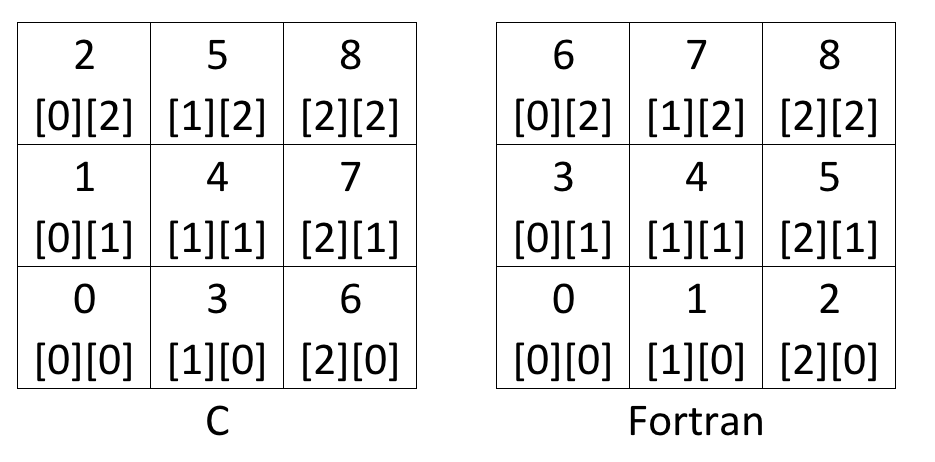
\includegraphics[scale=0.4]{memory_layout.png}
					\caption{The memory layout of 2D arrays in both C and Fortran. Note how columns are contiguous in memory in C and rows are contiguous in Fortran. \textit{Note: the numbers 0-8 indicate the position in linear memory.}}
					\label{fig:memory_layout}
				\end{figure}
				
			Due to how columns in 2D arrays are contiguous in C, to send a row of an array between MPI processes, we have to define an MPI vector. If the program was written in Fortran, rows are contiguous in memory and we would instead need an MPI vector to send columns of an array to other processes; refer to Fig. \ref{fig:memory_layout} for a pictorial representation of how memory is stored. We thus have to use MPI vectors to send the bottom and top halo boundary cells at the start of each iteration. To define this vector, we define the vector using \texttt{count = nx\char`_proc}, \texttt{blocklength = 1} and \texttt{stride = ny\char`_proc + 2}. By defining a vector with these values, we ensure that we pick up one value every \texttt{ny\char`_proc + 2} elements, \texttt{nx\char`_proc} times, i.e. an entire row of the \texttt{old}, \texttt{new} or \texttt{edge} arrays for a process.	
				
		\subsection{Updating Halo Cells Between Processes}
			At the start of each iteration, we need to update the halo cells of the \texttt{old} array. To do this, two communication types were developed.
			
			The first communication method implements a series of non-blocking \texttt{MPI\char`_Issend} send and blocking \texttt{MPI\char`_Recv} receive communications; refer to the pseudocode in Fig. \ref{fig:communication}. As mentioned in the previous section, sending columns of data in C from an array with MPI is relatively straight forwards. In the program, the left most and right most columns, within the image boundary, of the \texttt{old} array are sent to the neighbouring processes' halo cells. In Fig. \ref{fig:communication}, lines 1 - 8 deal with sending the columns, where \texttt{nbrs[LEFT]} and \texttt{nbrs[RIGHT]} are left and right neighbouring process' ranks. As the left and right most columns are contiguous in memory, we can simply define the starting location of the send buffer (\texttt{[j] = [1]}) and tell \texttt{MPI\char`_Issend} to take a count of \texttt{ny\char`_proc} which will send the whole column, excluding the halo cells. However, when we are sending the top and bottom rows we have to use the row vector defined in \S\ref{sect:array_vector} as rows in C are not contiguous in memory. We are thus unable to simply define a starting point and tell \texttt{MPI\char`_Issend} to take \texttt{nx\char`_proc} elements and send this, as we will be sending a column of length \texttt{nx\char`_proc} instead. Thus, as can be seen in lines 9 - 16 in Fig. \ref{fig:communication}, we send and receive rows of an array using the vector \texttt{send\char`_halo\char`_vector}, where again the \texttt{nbrs} array has been used again with \texttt{nbrs[UP]} and \texttt{nbrs[DOWN]} being the ranks for the neighbouring up and down processes in the 2D topology.
						
			\begin{figure}
				\begin{minted}[frame=lines, framesep=2mm, gobble=5]{c}
					 1	 // send right hand column to halo cells
					 2	 MPI_Issend(&old[nx_proc][1], ny_proc, MPI_DOUBLE, &nbrs[RIGHT], ...)
					 3	 MPI_Recv(&old[0][1], ny_proc, MPI_DOUBLE, &nbrs[LEFT], ..)
					 4	 MPI_Wait(&proc_request, &recv_status)
					 5	 // send left hand column to halo cells
					 6	 MPI_Issend(&old[1][1], ny_proc, MPI_DOUBLE, &nbrs[LEFT], ...)
					 7	 MPI_Recv(&old[nx_proc+1][1], ny_proc, MPI_DOUBLE, &nbrs[RIGHT], ..)
					 8	 MPI_Wait(&proc_request, &recv_status)		
					 9	 // send top rows to halo cells
					10	MPI_Issend(&old[1][ny_proc], 1, send_halo_vector, &nbrs[UP], ...)
					11	MPI_Recv(&old[1][0], 1, send_halo_vector, &nbrs[DOWN], ..)
					12	MPI_Wait(&proc_request, &recv_status)
					13	// send bottom rows to halo cells
					14	MPI_Issend(&old[1][1], 1, send_halo_vector, &nbrs[DOWN], ...)
					15	MPI_Recv(&old[1][ny_proc+1], 1, send_halo_vector, &bnrs[UP], ..)
					16	MPI_Wait(&proc_request, &recv_status)		
				\end{minted}
				\caption{Pseudocode for the non-blocking send and blocking receive communication used to send data to the halo cells of neighbouring processes.}
				\label{fig:communication}
			\end{figure}
			
			The second communication method implements a series of non-blocking send and receive communications. For this style, each send function is replaced with \texttt{MPI\char`_Isend} and the receive functions are replaced with \texttt{MPI\char`_Irecv}. We will also require the use of an \texttt{MPI\char`_Waitall} function at the end of communication. Example pseudocode can be found in Fig. \ref{fig:communication2}. The benefit of using this communication style is that the send and receive functions will return immediately which results in processes being able to move on immediately to the next send and receive communication. However, processes are now required to wait at the end for all communications to be complete, which is controlled by a \texttt{MPI\char`_Waitall} function. The datatypes, and their counts, used in the previous communication style will remain the same. 
			
			\begin{figure}
				\begin{minted}[frame=lines, framesep=2mm, gobble=4]{c}
				1	 // send right hand column to halo cells
				2	 MPI_Issend(&old[nx_proc][1], ny_proc, MPI_DOUBLE, RIGHT_PROC, ...)
				3	 MPI_Irecv(&old[0][1], ny_proc, MPI_DOUBLE, LEFT_PROC, ..)
				4	 // send left hand column to halo cells
				5	 MPI_Issend(&old[1][1], ny_proc, MPI_DOUBLE, LEFT_PROC, ...)
				6	 MPI_Irecv(&old[nx_proc+1][1], ny_proc, MPI_DOUBLE, RIGHT_PROC, ..)
				7	 // send top rows to halo cells
				8	 MPI_Issend(&old[1][ny_proc], 1, send_halo_vector, UP_PROC, ...)
				9	 MPI_Irecv(&old[1][0], 1, send_halo_vector, DOWN_PROC, ..)
				10	MPI_Wait(&proc_request, &recv_status)
				11	// send bottom rows to halo cells
				12	MPI_Issend(&old[1][1], 1, send_halo_vector, DOWN_PROC, ...)
				13	MPI_Irecv(&old[1][ny_proc+1], 1, send_halo_vector, UP_PROC, ..)
				14	// wait for all communication to end
				15	MPI_Wait(&proc_requests, &wait_status)		
				\end{minted}
				\caption{Pseudocode for a non-blocking send and non-blocking receive communication routine to send data to the halo cells of neighbouring processes.}
				\label{fig:communication2}
			\end{figure}
			
			Both methods of communication are functional, however, the combination of both non-blocking send and receives is expected to be more efficient due to less blocking operations and thus, this is the preferred method.
			
		\subsection{MPI Datatype - Array Vector} \label{sect:array_vector}
			To send subsections, or whole arrays, in one fell swoop we can utilise the MPI derived datatype, \texttt{MPI\char`_Vector}. This datatype is used when gathering work from processes to the master process, i.e. sending \texttt{buff} to \texttt{masterbuff}. Using this vector allows the arrays to be sent as one chunk and makes the algorithm more readable. To define this vector, we define \texttt{count = nx\char`_proc}, \texttt{blocklength = ny\char`_proc} and \texttt{stride = ny}, i.e. we collect a memory chunk of \texttt{ny\char`_proc}'s, every \texttt{ny} block of memory, \texttt{nx\char`_proc} times. This translates to grabbing a column of length \texttt{ny\char`_proc}, \texttt{nx\char`_proc} or an array of size \texttt{nx\char`_proc} x \texttt{ny\char`_proc}.	
		
		\subsection{Gathering Work and Reconstructing the Image} \label{sect:reconstruct}
			Once all iterations are complete, or if the difference between iterations is sufficiently small, each process' \texttt{buff} needs to be merged back into the \texttt{masterbuff} to reconstruct the image. Each process copies the array \texttt{old} into their \texttt{buff} arrays. If \texttt{NDIMS=1}, the MPI function \texttt{MPI\char`_Gather} is used to gather all of the \texttt{buff}'s back into \texttt{masterbuff} on the master process. However, when \texttt{NDIMS=2}, the \texttt{buff}'s (apart from the master process' \texttt{buff}) are synchronously sent to the master process. The master process is able to copy \texttt{buff} into \texttt{masterbuff} directly and receives \texttt{buff} from the other processes through an \texttt{MPI\char`_Recv} function, using the vector datatype described in \S\ref{sect:array_vector}, for each of the other processes. The process' \texttt{buff} are copied to the correct region of \texttt{masterbuff} by indexing the receive buffer using \texttt{nx\char`_proc\char`_start} and \texttt{ny\char`_proc\char`_start} similarly to how the image is de-constructed as described in \S\ref{sect:deconstruct}.

	\section{Correctness Tests and Parallel Scaling}
		The performance of the code in parallel is tested using four images with resolutions, 192 x 128, 256 x 192, 512 x 384 and 768 x 768. By using a range of resolutions, we will be able to examine how parallel image processing scales with resolution and number of processes. Ttests were conducted on ARCHER using 1, 2, 4, 8, 16, 24, 48, 72, 96 and 120 processes. 

		\subsection{Image Output}
			\begin{table}[h]
				\centering
				\begin{tabular}{|c|c|}
					\hline
					\textbf{Resolution} & \textbf{Average Iterations to Complete} \\ \hline
					192 x 128           & 1500                                    \\
					252 x 192           & 1100                                    \\
					512 x 384           & 1500                                    \\
					768 x 768           & 1300                                    \\ \hline
				\end{tabular}
				\caption{The number of iterations required to reconstruct the original image for each image resolution tested.}
				\label{tab:iterations}
			\end{table}
		
			Fig. \ref{fig:before_after_images} shows an example of the input and output of the program using the 192 x 128 and the 768 x 768 edge images. As can be seen, both images were reconstructed successfully and both took around 1400 iterations before \texttt{DELTA = 0.1} was satisfied; the number of iterations computed for the other images can be found in Table \ref{tab:iterations}. Image quality/accuracy did not change with the number of processes in use and a visual comparison of the output between the parallel and serial versions showed that the tests images were being converted correctly. The highest resolution image has a rather odd, uneven lighting to it. There is a halo of white light surrounding the structure of the castle and the hill. However, as I did not have access to the image before it was converted into an edge image, I am unable to pinpoint if the cause of this halo of light; also present in the serial version. It could be due to the reconstruction algorithm or the original image could have just been like this.
					
			\begin{figure}
				\centering
				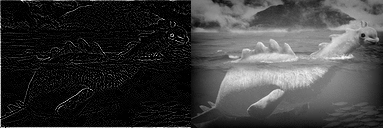
\includegraphics[scale=1.2]{image1.png}
				~\\~\\
				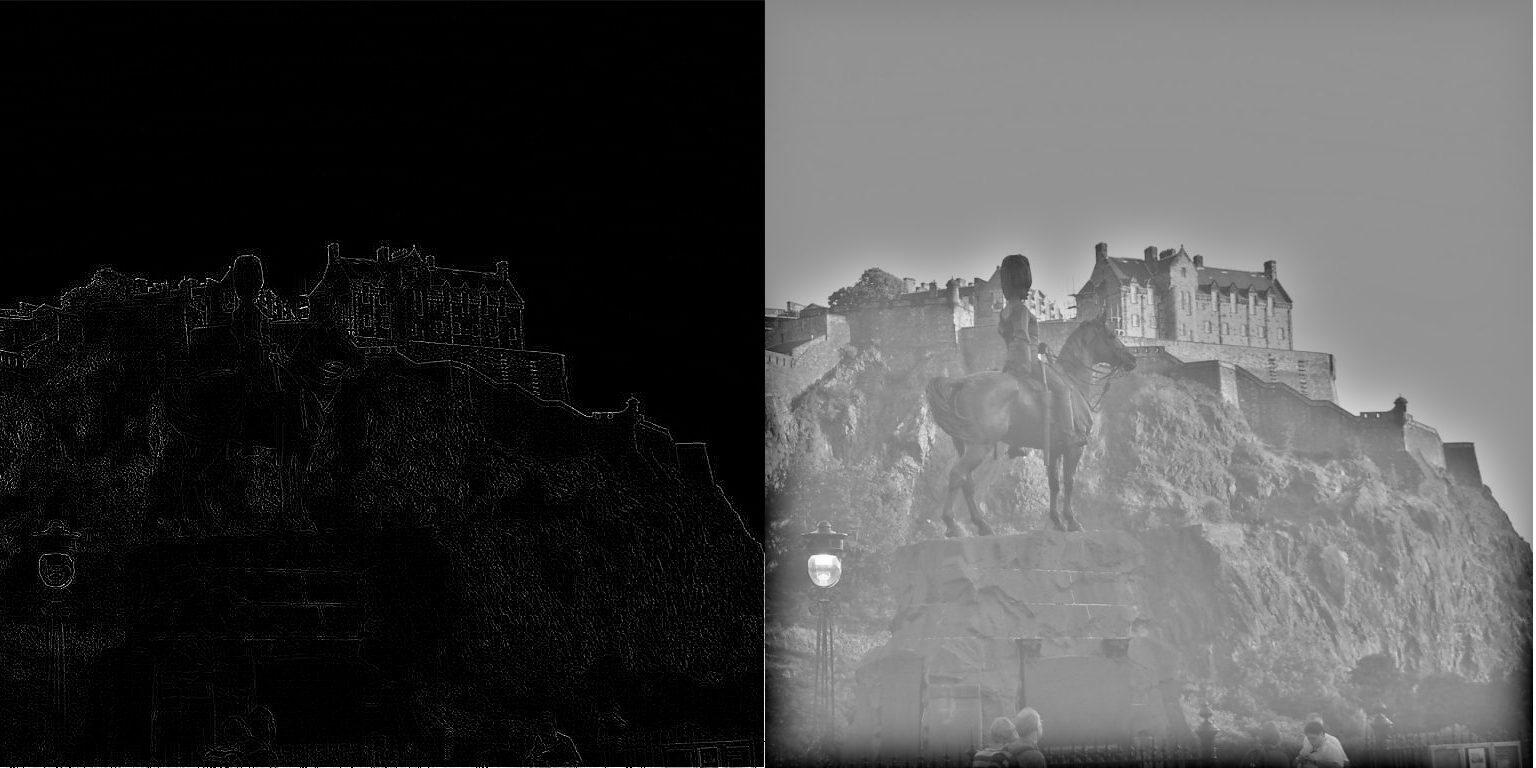
\includegraphics[scale=0.3]{image4.png}
				\caption{The dark images on the left correspond to the edge images that the program aims to convert. The images on the right, the Loch Ness monster (top) and Edinburgh Castle (bottom), are the reconstructed images. Both took around 1500 iterations to satisfy the criterion \texttt{DELTA = 0.1}.}
				\label{fig:before_after_images}
			\end{figure}

		\subsection{Parallel Scaling}	
			\begin{figure}
				\centering
				\includegraphics[scale=0.38]{results/np_speedup.pdf}
				\includegraphics[scale=0.38]{results/np_periter.pdf}
				\caption{Top: the speed up factor of the conversion iterations against the number of processes in use, for all four image resolutions. Bottom: the average time per conversion iteration against the number of process in use, for all four image resolutions.}
				\label{fig:np_runtime}
			\end{figure}
		
		\textit{Tables \ref{tab:all_data1} and \ref{tab:all_data} in \S\ref{sect:appendix} include all run times data collected for the parallel scaling tests.}
		
	\section{Conclusion}
		
	\newpage
	\section{Appendix} \label{sect:appendix}
		\begin{sidewaystable}
		  \centering
		   	\begin{tabular}{|c|c|c|c|c|c|c|c|}
				\hline
				\multicolumn{1}{|p{7.5em}|}{\textbf{Resolution}} & \multicolumn{1}{p{7.5em}|}{\textbf{Number of Processes}} & \multicolumn{1}{p{7.5em}|}{\textbf{Total Iteration Time (ms)}} & \multicolumn{1}{p{7.5em}|}{\textbf{Average Iteration Time per Process (ms)}} & \multicolumn{1}{p{7.5em}|}{\textbf{Average Time Per Iteration (ms)}} & \multicolumn{1}{p{7.5em}|}{\textbf{Time for Domain Composition (ms)}} & \multicolumn{1}{p{7.5em}|}{\textbf{Time for Domain Reconstruction (ms)}} & \multicolumn{1}{p{7.5em}|}{\textbf{Total Runtime (ms)}} \\
				\hline
				\textbf{192 x 128} & 1     & 129.8720 & 129.8720 & 0.0866 & 0.1690 & 0.0450 & 246.2720\\
				\textbf{192 x 128} & 2     & 65.9760 & 32.9870 & 0.0440 & 0.1290 & 0.1000 & 193.2920 \\
				\textbf{192 x 128} & 4     & 38.2990 & 9.5740 & 0.0255 & 0.0820 & 0.1560 & 163.1950 \\
				\textbf{192 x 128} & 8     & 24.9400 & 3.1180 & 0.0166 & 0.0240 & 0.2140 & 295.7200 \\
				\textbf{192 x 128} & 16    & 18.4340 & 1.1520 & 0.0123 & 0.0260 & 0.3740 & 397.7480 \\
				\textbf{192 x 128} & 24    & 17.0200 & 0.7090 & 0.0113 & 0.0080 & 0.2910 & 543.6620 \\
				\textbf{192 x 128} & 48    & 28.4090 & 0.5920 & 0.0189 & 0.0050 & 5.6760 & 754.6030 \\
				\textbf{192 x 128} & 72    & 39.7830 & 0.5530 & 0.0265 & 0.0030 & 3.7380 & 871.7760 \\
				\textbf{192 x 128} & 96    & 53.6050 & 0.5580 & 0.0357 & 0.0030 & 5.3410 & 828.1630 \\
				\textbf{192 x 128} & 120   & 91.4060 & 0.7620 & 0.0609 & 0.0020 & 5.9220 & 752.6720 \\
				\hline
				\textbf{256 x 192} & 1     & 190.9390 & 190.9390 & 0.1736 & 0.5770 & 0.0730 & 301.7730 \\
				\textbf{256 x 192} & 2     & 99.0180 & 49.5090 & 0.0900 & 0.2840 & 0.1690 & 180.5140 \\
				\textbf{256 x 192} & 4     & 53.3280 & 13.3320 & 0.0485 & 0.1170 & 0.1760 & 211.3410 \\
				\textbf{256 x 192} & 8     & 31.3200 & 3.9150 & 0.0285 & 0.0600 & 0.3050 & 255.4980 \\
				\textbf{256 x 192} & 16    & 20.8250 & 1.3020 & 0.0189 & 0.0250 & 0.4320 & 437.0170 \\
				\textbf{256 x 192} & 24    & 17.5710 & 0.7320 & 0.0160 & 0.0180 & 0.3550 & 574.5650 \\
				\textbf{256 x 192} & 48    & 19.1110 & 0.3980 & 0.0174 & 0.0070 & 4.9100 & 607.8310 \\
				\textbf{256 x 192} & 72    & 20.9860 & 0.2910 & 0.0191 & 0.0080 & 6.2710 & 639.4050 \\
				\textbf{256 x 192} & 96    & 53.0420 & 0.5530 & 0.0482 & 0.0030 & 3.8940 & 694.1410 \\
				\textbf{256 x 192} & 120   & 57.8550 & 0.4820 & 0.0526 & 0.0040 & 6.5600 & 693.0820 \\
				\hline
			\end{tabular}
		  \caption{Results from the runtime tests for the 192 x 128 and 256 x 192 images.}
		  \label{tab:all_data1}
		  
		\end{sidewaystable}	
		\begin{sidewaystable}
			\centering
			    \begin{tabular}{|c|c|c|c|c|c|c|c|}
					\hline
					\multicolumn{1}{|p{7.5em}|}{\textbf{Resolution}} & \multicolumn{1}{p{7.5em}|}{\textbf{Number of Processes}} & \multicolumn{1}{p{7.5em}|}{\textbf{Total Iteration Time (ms)}} & \multicolumn{1}{p{7.5em}|}{\textbf{Average Iteration Time per Process (ms)}} & \multicolumn{1}{p{7.5em}|}{\textbf{Average Time Per Iteration (ms)}} & \multicolumn{1}{p{7.5em}|}{\textbf{Time for Domain Composition (ms)}} & \multicolumn{1}{p{7.5em}|}{\textbf{Time for Domain Reconstruction (ms)}} & \multicolumn{1}{p{7.5em}|}{\textbf{Total Runtime (ms)}} \\
					\hline
					\textbf{512 x 384} & 1     & 1034.7620 & 1034.7620 & 0.6898 & 1.5040 & 0.2490 & 1296.6220 \\
					\textbf{512 x 384} & 2     & 528.8800 & 264.4400 & 0.3526 & 1.0810 & 0.4460 & 673.9290 \\
					\textbf{512 x 384} & 4     & 282.6000 & 70.6500 & 0.1884 & 0.3910 & 0.6260 & 433.3400 \\
					\textbf{512 x 384} & 8     & 150.0970 & 18.7620 & 0.1001 & 0.2050 & 0.7940 & 437.8820 \\
					\textbf{512 x 384} & 16    & 82.3340 & 5.1460 & 0.0549 & 0.1230 & 0.8800 & 485.8020 \\
					\textbf{512 x 384} & 24    & 57.4650 & 2.3940 & 0.0383 & 0.0780 & 0.9120 & 627.1880 \\
					\textbf{512 x 384} & 48    & 44.9670 & 0.9370 & 0.0300 & 0.0930 & 6.5260 & 774.1110 \\
					\textbf{512 x 384} & 72    & 71.6520 & 0.9950 & 0.0478 & 0.0410 & 7.4380 & 949.9000 \\
					\textbf{512 x 384} & 96    & 59.9300 & 0.6240 & 0.0400 & 0.0460 & 7.9480 & 718.3170 \\
					\textbf{512 x 384} & 120   & 75.4580 & 0.6290 & 0.0503 & 0.0170 & 8.4920 & 766.2610[b]\\
					\hline
					\textbf{768 x 768} & 1     & 2688.7330 & 2688.7320 & 2.0683 & 5.5930 & 0.8410 & 2919.5260 \\
					\textbf{768 x 768} & 2     & 1366.5360 & 683.2680 & 1.0512 & 3.1350 & 1.6620 & 1701.0110 \\
					\textbf{768 x 768} & 4     & 717.4920 & 179.3730 & 0.5519 & 1.5210 & 1.8300 & 1224.6340 \\
					\textbf{768 x 768} & 8     & 372.6510 & 46.5810 & 0.2867 & 0.9220 & 2.0560 & 1122.0540 \\
					\textbf{768 x 768} & 16    & 199.7100 & 12.4820 & 0.1536 & 0.3830 & 2.3410 & 1040.0760 \\
					\textbf{768 x 768} & 24    & 136.0880 & 5.6700 & 0.1047 & 0.2160 & 2.3360 & 874.5660 \\
					\textbf{768 x 768} & 48    & 127.9420 & 2.6650 & 0.0984 & 0.1090 & 7.4290 & 1686.0230 \\
					\textbf{768 x 768} & 72    & 83.6020 & 1.1610 & 0.0643 & 0.1090 & 10.3440 & 1561.1830 \\
					\textbf{768 x 768} & 96    & 74.4630 & 0.7760 & 0.0573 & 0.0750 & 10.3610 & 1506.8010 \\
					\textbf{768 x 768} & 120   & 128.8720 & 1.0740 & 0.0991 & 0.1330 & 10.1450 & 1033.0560 \\
				\hline
			\end{tabular}
		\caption{Results from the runtime tests for the 1512 x 384 and 768 x 768 images.}
		\label{tab:all_data}
	\end{sidewaystable}
		
\end{document}